\documentclass{article}%
\usepackage{amsmath}%
\usepackage{amsfonts}%
\usepackage{amssymb}%
\usepackage{graphicx}
\usepackage{sectsty}
\usepackage{listings}
\usepackage{framed}
\usepackage{color}
\usepackage{verbatim}
\usepackage{graphicx} %插入图片的宏包
\usepackage{float} %设置图片浮动位置的宏包
\usepackage{subfigure} %插入多图时用子图显示的宏包
\definecolor{shadecolor}{rgb}{.9, .9, .9}
\sectionfont{\fontsize{20}{20}\selectfont}
%-------------------------------------------
\newtheorem{theorem}{Theorem}
\newtheorem{acknowledgement}[theorem]{Acknowledgement}
\newtheorem{algorithm}[theorem]{Algorithm}
\newtheorem{axiom}[theorem]{Axiom}
\newtheorem{case}[theorem]{Case}
\newtheorem{claim}[theorem]{Claim}
\newtheorem{conclusion}[theorem]{Conclusion}
\newtheorem{condition}[theorem]{Condition}
\newtheorem{conjecture}[theorem]{Conjecture}
\newtheorem{corollary}[theorem]{Corollary}
\newtheorem{criterion}[theorem]{Criterion}
\newtheorem{definition}[theorem]{Definition}
\newtheorem{example}[theorem]{Example}
\newtheorem{exercise}[theorem]{Exercise}
\newtheorem{lemma}[theorem]{Lemma}
\newtheorem{notation}[theorem]{Notation}
\newtheorem{problem}[theorem]{Problem}
\newtheorem{proposition}[theorem]{Proposition}
\newtheorem{remark}[theorem]{Remark}
\newtheorem{solution}[theorem]{Solution}
\newtheorem{summary}[theorem]{Summary}
\newenvironment{proof}[1][Proof]{\textbf{#1.} }{\ \rule{0.5em}{0.5em}}
\setlength{\textwidth}{7.0in}
\setlength{\oddsidemargin}{-0.35in}
\setlength{\topmargin}{-0.5in}
\setlength{\textheight}{30.0in}
\setlength{\parindent}{0.3in}

\newenvironment{code}%
   {\snugshade\verbatim}%
   {\endverbatim\endsnugshade}

\begin{document}

\begin{flushright}
\begin{LARGE}

\textbf{Zhuang Liu \\
SID: 25727277}
\end{LARGE}
\end{flushright}

\begin{center}
\begin{huge}
\textbf{CS 230 Distributed Computer Systems \\
Homework 2} \\
\end{huge}
\end{center}

\section{The Approach}
\begin{Large}

In this assignment, we need two programs to simulate the communication process between two devices. Let's name the two programs after sender and receiver. To transport message between devices, we need socket APIs provided by Python in both sender and receiver programs.
\begin{code}
    import socket, sys
\end{code}
\begin{flushleft}
\begin{LARGE}
\textbf{1.1 Sender Side Construction}
\end{LARGE}
\end{flushleft}

When implementing the \texttt{main} function, we should do two things: build the socket, which serves as a bridge passing message between the sender and the receiver; After built up the socket, we can begin to listen to the receiver to get receiver's information and send data to the receiver.

\begin{flushleft}
\textbf{1.1.1 Building the Socket}
\end{flushleft}

At first, we can initialize a listening socket for sender utilizing Python's socket APIs. Here, the \texttt{AF\_INET} refers to the IPv4 address, the \texttt{SOCK\_STREAM} means connection oriented TCP protocol. 

\begin{code}
    sender_socket = socket.socket(socket.AF_INET,socket.SOCK_STREAM)
\end{code}

Then, we should bind the socket to some IP address and well-known ports. If we want to bind to all available IP addresses, we should specify \texttt{0.0.0.0} as our IP address, which will make the routing in this program easier. I also choose the port number \texttt{8080}.

\begin{code}
    sender_socket.bind(('0.0.0.0', 8080))
\end{code}

Since we are building a one-to-one sender-receiver model, we will set the maximum connection number of the \texttt{sender\_socket} to 1.

\begin{code}
    sender_socket.listen(1)
\end{code}

\newpage

Now we can say the socket of the sender is built up and open to use.

\begin{flushleft}
\textbf{1.1.2 Communication with the Receiver}
\end{flushleft}

Here, I build a thread to execute the process. The further implementation will be inside the following loop:

\begin{code}
    while True:
\end{code}

By listening to the receiver, we can get the receiver's connection and address.

\begin{code}
    receiver_connection, receiver_address = sender_socket.accept()
\end{code}

Then, since we only need to transport a short string, the size of the string won't be too large. We can set the maximum size of the receiver's data to \texttt{1024}. By the mean time, we can get the receiver's data here.

\begin{code}
    data = receiver_connection.recv(1024)
\end{code}

Now we get the receiver's data. In order to check if the process is successful, we can print the data to the console.

\begin{code}
    print("Data from the Receiver: %s" % (data))
\end{code}

After listening to the receiver, we can send our message to the receiver through the socket.

\begin{code}
    message = "Good"
    receiver_connection.send(message.encode())
\end{code}

After sending the message, we can close the socket now.

\begin{code}
    receiver_connection.close()
\end{code}

At this stage, the thread is ended. We can close the sender and quit the program now.

\begin{code}
    sender_socket.close()
    sys.exit()
\end{code}

\newpage

\begin{LARGE}
\begin{flushleft}
\textbf{1.2 Receiver Side Construction}
\end{flushleft}
\end{LARGE}

To build the receiver program, the general steps are analogous to the sender side construction. Here is the way to implement the \texttt{main} function. At first we build the socket between sender and receiver, then send request to the sender, after sender sent its message, we retrieve that message then close our receiver.

\begin{flushleft}
\textbf{1.2.1 Building the Socket}
\end{flushleft}

At first, we should initialize the socket:

\begin{code}
    receiver_socket = socket.socket(socket.AF_INET,socket.SOCK_STREAM)
\end{code}

Then, by convenience, we can set the public IPv4 address to \texttt{10.211.55.4} (ip address of interface \texttt{enp0s5} on my Ubuntu Linux), and port number \texttt{8080}, and connect the socket.

\begin{code}
    receiver_socket.connect(('10.211.55.4', 8080))
\end{code}

\begin{flushleft}
\textbf{1.2.2 Communication with the Sender}
\end{flushleft}

After building the socket, we can send our request to the sender to get its message.

\begin{code}
    request = "GET MSG"
    receiver_socket.send(request.encode())
\end{code}

By then, if the sender get our request, it will send a message to the receiver, now we are going to retrieve the message from the sender:

\begin{code}
    message = receiver_socket.recv(1024).decode()
\end{code}

To see if we get the message successfully, we can print the message out on the console:

\begin{code}
    print("Message from the Sender %s" % (message))
\end{code}

Now we accomplished the communication between sender and server, we can close the receiver socket and quit the program:

\begin{code}
    receiver_socket.close()
    sys.exit()
\end{code}

\end{Large}
\newpage

\section{Wireshark Packet Analysis}
\begin{Large}

\begin{LARGE}
\begin{flushleft}
\textbf{2.1 Building the Environment}
\end{flushleft}
\end{LARGE}

I deployed the \texttt{sender.py} program on a \texttt{Ubuntu Linux 18.04} device(\texttt{Ubuntu}), and the \texttt{receiver.py} program on a \texttt{macOS Mojave 10.14.2} device(\texttt{Mac}).

From the \texttt{Ubuntu}, we can start wireshark by running shell script:
\begin{code}
    wireshark
\end{code}
We can get the IP address of the \texttt{Ubuntu} by:
\begin{code}
    ifconfig
\end{code}
So now we get the IP address of the \texttt{Ubuntu}, which is \texttt{10.211.55.2}. With this address, we can add a capture filter entry in wireshark to isolate the packets corresponding to the communication between the \texttt{sender.py} and the \texttt{receiver.py}.
\begin{code}
    To 10.211.55.2 | ip.dst == 10.211.55.2
\end{code}
With wireshark set up, we can start \texttt{sender.py} on \texttt{Ubuntu}:
\begin{code}
    python2 sender.py
\end{code}
Then, start \texttt{receiver.py} on \texttt{Mac}:
\begin{code}
    python2 receiver.py
\end{code}

\begin{LARGE}
\begin{flushleft}
\textbf{2.2 Network Analysis}
\end{flushleft}
\end{LARGE}

After setting up the environment and launching the sender and receiver, we can get the captured packets in wireshark.
\begin{center}
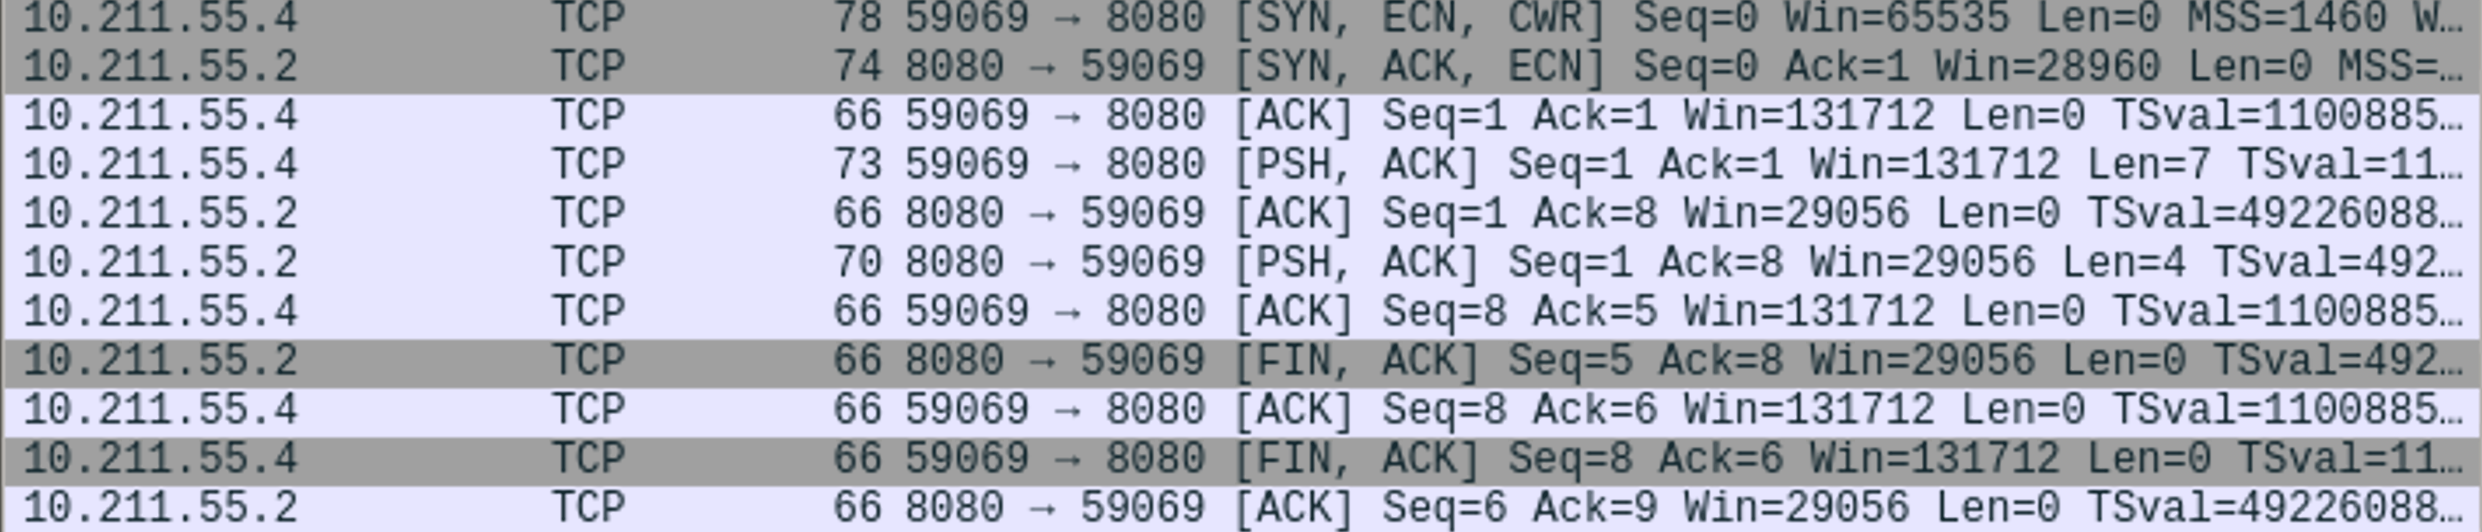
\includegraphics[width=1.0\textwidth]{wireshark.png}
\end{center}
\newpage
By opening the fifth packet, we can see the byte information inside the packet. Using the interpreter inside wireshark, we can answer the following questions.
\newline
1. What is encoded in bytes 0-5 and 6-11?
\newline
0-5: Destination MAC address(Globally unique address and Individual address)
\begin{code}
    Address: Parallel_00:00:08 (00:1c:42:00:00:08)
\end{code}
\newline
\begin{flushleft}
6-11: Source MAC address
\end{flushleft}
\begin{code}
    Address: Parallel_27:07:24 (00:1c:42:27:07:24)
\end{code}
2. What is encoded in, and what is the relationship between, byte 14 and the two bytes 16-17?
\begin{flushleft}
14: The header length of the message
\end{flushleft}
\begin{code}
    0101 = Header Length: 20 bytes (5)
\end{code}
\begin{flushleft}
16-17: Total length of the message
\end{flushleft}
\begin{code}
    Total length: 52
\end{code}
Header is pointing to the beginning of the data, header length is the length of the header. While total length is the length of the whole datagram. Header length is a part of the total length.
\begin{flushleft}
3. What is encoded in bytes 18-19?
\newline
18-19: Identification of IPv4
\end{flushleft}
\begin{code}
    Identification: 0x1b12(6930)
\end{code}
\begin{flushleft}
4. What is encoded in bytes 20-21?
\newline
20-21: Fragment offset of the Flag of the IPv4
\end{flushleft}
\begin{code}
    ...0 0000 0000 0000 = Fragment offset: 0
\end{code}
\begin{flushleft}
5. What is encoded in byte 23?
\newline
23: Protocol Type
\end{flushleft}
\begin{code}
    Protocol: TCP(6)
\end{code}
\newpage
\begin{flushleft}
6. What is encoded in bytes 26-29 and 30-33?
\newline
26-29: Source address in the header
\end{flushleft}
\begin{code}
    Source: 10.211.55.4
\end{code}

\begin{flushleft}
30-33: Destination address in the header
\end{flushleft}
\begin{code}
    Destination: 10.211.55.2
\end{code}
\begin{flushleft}
7. What is encoded in bytes 34-35 and 36-37?
\newline
34-35: Source port
\end{flushleft}
\begin{code}
    Source Port: 8080
\end{code}
\begin{flushleft}
36-37: Destination Port
\end{flushleft}
\begin{code}
    Destination Port: 59069
\end{code}
\begin{flushleft}
8. What is encoded after byte 65?
\newline
66-...: App header and user data
\end{flushleft}
\begin{code}
    NULL
\end{code}

\begin{LARGE}
\begin{flushleft}
\textbf{2.3 Layer Classification}
\end{flushleft}
\end{LARGE}
\begin{flushleft}
\textbf{2 Link Layer}
\begin{code}
    0-5
    6-11 
\end{code}

\textbf{3 Network Layer}
\begin{code}
    14
    16-17
    18-19
    20-21
    23
    26-29
    30-33
\end{code}
\newpage
\textbf{4 Transport Layer}
\begin{code}
    34-35
    36-37
\end{code}
\textbf{7 Application Layer}
\begin{code}
    66-...
\end{code}
\end{flushleft}

\end{Large}
\section{File Listing}
\begin{Large}
In \texttt{Ubuntu}, the structure of key files of this project can be interpreted as follows:
\begin{code}
    sender.py
    \packets
        capture.pcapng
\end{code}
In \texttt{Mac}, the structure of key files of this project can be interpreted as follows:
\begin{code}
    receiver.py
\end{code}
\end{Large}

\end{document}